\documentclass[12pt]{book} % Change to book
\usepackage{amsmath} % For mathematical expressions
\usepackage{xcolor} % For colored text
\usepackage{graphicx} % For including images
\usepackage{url}
\usepackage{booktabs} % For better-looking tables
\usepackage{makecell}
\usepackage{indentfirst}
\usepackage{algorithm}
\usepackage{algpseudocode}
\usepackage{amssymb}
\usepackage{placeins} % For \FloatBarrier
\usepackage{listings}
% Define the language style For Python code
\lstset{
    language=Python,
    basicstyle=\ttfamily,
    keywordstyle=\color{blue},
    stringstyle=\color{red},
    commentstyle=\color{gray},
    morecomment=[l][\color{magenta}]{\#},
    frame=single,
    breaklines=true
}
\begin{document}

\chapter{Greedy Algorithms}

\section{Introduction to Greedy Algorithms}
Greedy algorithms are a neat way to solve problems by always making the best choice at the moment. Think of it like picking the ripest fruit each time from a basket to hopefully end up with the best bunch at the end. These algorithms build up solutions step by step, choosing options that seem the best at each step. They work really well for certain types of problems where each of these choices leads us closer to an optimal solution, although they might not always give the perfect answer for every scenario.

\textbf{Algorithmic example with mathematical detail in LaTeX:}
\FloatBarrier

\begin{algorithm}
\caption{Greedy Algorithm Example}
\begin{algorithmic}[1]
\State Assume we have a set of $n$ tasks $T = \{t_1, t_2, \ldots, t_n\}$ with respective profits $P = \{p_1, p_2, \ldots, p_n\}$ and deadlines $D = \{d_1, d_2, \ldots, d_n\}$.
\State Sort tasks based on their profits in decreasing order.
\State Initialize schedule $S$ as an empty list.
\For{$i$ from $1$ to $n$}
    \State Insert task $t_i$ into $S$ at the latest possible position without missing its deadline.
\EndFor
\State \textbf{Return} Schedule $S$ with maximum total profit.
\end{algorithmic}
\end{algorithm}
\FloatBarrier

\textbf{Python code equivalent For the algorithmic example:}
\FloatBarrier
\begin{lstlisting}
def greedy_schedule(tasks):
    tasks.sort(key=lambda x: x[1], reverse=True)  # Sort tasks by profit in decreasing order
    schedule = []
    n = len(tasks)
    For i in range(n):
        deadline = tasks[i][2]
        while deadline > 0 and deadline <= n:  # Insert task at latest possible position without missing deadline
            if deadline not in [x[0] For x in schedule]:
                schedule.append(tasks[i])
                break
            deadline -= 1
    Return schedule

# Example tasks Format: 

(task_id, profit, deadline)
tasks = [(1, 40, 2), (2, 35, 1), (3, 30, 3), (4, 25, 1), (5, 20, 3)]
print(greedy_schedule(tasks))
\end{lstlisting}
\FloatBarrier

\subsection{Definition and Characteristics}
Greedy algorithms make a series of decisions, where each decision selects the locally optimal choice at that step. The hope is that by picking a locally optimal solution at each step, the algorithm will eventually come up with a global optimum solution.

\textbf{Algorithmic Example: Coin Change Problem}

Let's consider the coin change problem where we want to find the minimum number of coins needed to make a certain amount. We are given a set of coin denominations and we need to Return the minimum number of coins that make up the desired amount.
\FloatBarrier
\begin{algorithm}
\caption{Greedy Coin Change Algorithm}
\begin{algorithmic}
\Function{GreedyCoinChange}{amount, coins}
    \State Initialize $change \gets []$
    \State Sort $coins$ in descending order
    \For {coin in $coins$}
        \State $numCoins \gets \lfloor \frac{amount}{coin} \rfloor$
        \State $change.append(numCoins)$
        \State $amount \gets amount - numCoins \times coin$
    \EndFor
    \State \Return $sum(change)$
\EndFunction
\end{algorithmic}
\end{algorithm}
\FloatBarrier
The python code equivalent For the Greedy Coin Change Algorithm is as follows:
\FloatBarrier
\begin{lstlisting}
def greedy_coin_change(amount, coins):
    change = []
    coins.sort(reverse=True)
    For coin in coins:
        numCoins = amount // coin
        change.append(numCoins)
        amount -= numCoins * coin
    Return sum(change)
\end{lstlisting}
\FloatBarrier


\textbf{Characteristics of Greedy Algorithms:}
\begin{itemize}
    \item \textbf{Greedy-choice Property}: At each step, a greedy algorithm makes a locally optimal choice that leads to the best possible solution For that step without considering the overall outcome.
    \item \textbf{Optimal Substructure}: The optimal solution to the problem can be obtained by combining the locally optimal choices made at each step.
    \item \textbf{Does not reconsider choices}: Once a decision is made, a greedy algorithm does not revisit or reconsider it. This makes the algorithm efficient but may not always lead to the globally optimal solution
\end{itemize}

\subsection{Principles of Greedy Strategy}
The Greedy Strategy is a simple approach to solving optimization problems by making locally optimal choices at each step with the hope of finding a global optimum. The main principles of the Greedy Strategy are:

\begin{itemize}
    \item \textbf{Greedy Choice Property:} A globally optimal solution can be reached by making a locally optimal choice at each step.
    \item \textbf{Optimal Substructure:} The problem can be broken down into smaller subproblems, and the solution to the overall problem can be constructed from solutions to the subproblems.
\end{itemize}

One classic example of the Greedy Strategy is the \textbf{Coin Change Problem}. Given a set of coin denominations and a target amount, the goal is to find the minimum number of coins needed to make up that amount.

\textbf{Algorithm: Coin Change Problem}
\FloatBarrier
\begin{algorithm}
\caption{Greedy Coin Change Algorithm}
\begin{algorithmic}[1]
\Procedure{GreedyCoinChange}{$\text{coins}[], \text{target}$}
    \State $\text{numCoins} \gets 0$
    \State $\text{index} \gets \text{length}(\text{coins}) - 1$
    \While{$\text{target} > 0$ and $\text{index} \geq 0$}
        \If{$\text{coins}[\text{index}] \leq \text{target}$}
            \State $\text{numCoins} \gets \text{numCoins} + \text{target} \div \text{coins}[\text{index}]$
            \State $\text{target} \gets \text{target} \% \text{coins}[\text{index}]$
        \EndIf
        \State $\text{index} \gets \text{index} - 1$
    \EndWhile
    \State \textbf{Return} $\text{numCoins}$
\EndProcedure
\end{algorithmic}
\end{algorithm}
\FloatBarrier
\textbf{Python Code Equivalent:}
\FloatBarrier
\begin{lstlisting}
def greedy_coin_change(coins, target):
    numCoins = 0
    index = len(coins) - 1
    
    while target > 0 and index >= 0:
        if coins[index] <= target:
            numCoins += target // coins[index]
            target %= coins[index]
        index -= 1
        
    Return numCoins

\end{lstlisting}
\FloatBarrier
\textbf{Explanation:}
\begin{itemize}
    \item We start with the highest denomination coin and keep subtracting it from the target amount until it becomes zero or negative.
    \item Then, we move to the next smaller denomination and repeat the process until we reach the smallest denomination or the target amount becomes zero.
    \item At each step, we make the locally optimal choice by choosing the largest denomination that doesn't exceed the remaining target amount.
\end{itemize}

\subsection{Applications and Limitations}
Greedy algorithms are often used in optimization problems where we make a series of choices that result in an optimal solution. One common application is in the scheduling of activities to maximize the number of activities that can be performed within a given time constraint.

\textbf{Algorithmic Example: Activity Selection Problem}
\FloatBarrier
Given a set of activities with start and finish times, the goal is to select the maximum number of non-overlapping activities.
\FloatBarrier
\begin{algorithm}
\caption{Activity Selection Problem}
\begin{algorithmic}[1]
\State Sort activities by finish time
\State Include the first activity in the solution
\For{each activity starting from the second}
    \If{activity start time is greater than or equal to the finish time of the previously selected activity}
        \State Include the activity in the solution
    \EndIf
\EndFor
\end{algorithmic}
\end{algorithm}
\FloatBarrier
\textbf{Python Code Equivalent:}
\begin{lstlisting}
def activity_selection(activities):
    sorted_activities = sorted(activities, key=lambda x: x[1])
    selected_activities = [sorted_activities[0]]
    
    For activity in sorted_activities[1:]:
        if activity[0] >= selected_activities[-1][1]:
            selected_activities.append(activity)
    
    Return selected_activities

activities = [(1, 4), (3, 5), (0, 6), (5, 7), (3, 9), (5, 9), (6, 10), (8, 11), (8, 12), (2, 14), (12, 16)]
print(activity_selection(activities)) 
\end{lstlisting}
\FloatBarrier
This example demonstrates the application of a greedy algorithm For solving the activity selection problem. The algorithm selects activities based on their finish times to maximize the number of non-overlapping activities that can be performed. The provided Python code implements this algorithm For the given set of activities.


Although greedy algorithms are simple and efficient, they may not always provide the optimal solution. Some common limitations of greedy algorithms include:
\begin{itemize}
    \item Greedy algorithms may not always guarantee the globally optimal solution.
    \item They may overlook certain choices that lead to a better solution in the future.
    \item Finding the optimal solution may require considering all possible choices, which greedy algorithms do not always do.
\end{itemize}

To illustrate the limitations of greedy algorithms, let's consider the Fractional Knapsack Problem. 

In this problem, we are given a set of items, each with a weight \( w_i \) and a value \( v_i \), and a knapsack with a maximum weight capacity \( W \). The goal is to fill the knapsack with items to maximize the total value while not exceeding the weight capacity. Unlike the 0/1 Knapsack Problem, where items cannot be divided, in the Fractional Knapsack Problem, we can take fractions of items.

The greedy strategy For the Fractional Knapsack Problem involves selecting items based on their value-to-weight ratios. At each step, we choose the item with the highest value-to-weight ratio and take as much of it as possible until the knapsack is full. However, the greedy approach may not always yield the optimal solution.

Let's demonstrate this with an algorithmic example:

\begin{algorithm}
\caption{Greedy Fractional Knapsack Algorithm}
\begin{algorithmic}[1]
\Procedure{FractionalKnapsack}{items[], W}
    \State Sort items by decreasing value-to-weight ratio
    \State totalValue $\gets$ 0
    \State remainingWeight $\gets$ W
    \For{item in items}
        \If{item.weight $\leq$ remainingWeight}
            \State totalValue $\gets$ totalValue + item.value
            \State remainingWeight $\gets$ remainingWeight - item.weight
        \Else
            \State fraction $\gets$ remainingWeight / item.weight
            \State totalValue $\gets$ totalValue + fraction $\times$ item.value
            \State remainingWeight $\gets$ 0
            \State \textbf{break}
        \EndIf
    \EndFor
    \State \textbf{Return} totalValue
\EndProcedure
\end{algorithmic}
\end{algorithm}

\textbf{Python code:}
\FloatBarrier
\begin{lstlisting}
def fractional_knapsack(items, W):
    # Sort items by decreasing value-to-weight ratio
    items.sort(key=lambda x: x[1] / x[0], reverse=True)
    
    total_value = 0
    remaining_weight = W
    
    # Iterate through items
    For weight, value in items:
        # If item's weight can fit into remaining weight
        if weight <= remaining_weight:
            total_value += value
            remaining_weight -= weight
        else:
            # Take fraction of item
            fraction = remaining_weight / weight
            total_value += fraction * value
            remaining_weight = 0
            break
            
    Return total_value

# Example usage:
items = [(20, 100), (30, 120)]  # List of (weight, value) tuples
W = 50  # Knapsack capacity
print("Total value:", fractional_knapsack(items, W))
\end{lstlisting}
\FloatBarrier

In this algorithm, \texttt{items} is a list of items with their respective weights and values. The algorithm sorts the items in decreasing order of their value-to-weight ratios and iterates through them. At each step, if the entire weight of the current item can fit into the knapsack, it is fully taken. Otherwise, a fraction of the item is taken to fill the remaining capacity.

However, the greedy approach fails For cases where the items' value-to-weight ratios do not reflect their overall contribution to the solution. Consider the following example:

Suppose we have a knapsack with a capacity of 50 units and the following items:

\begin{itemize}
    \item Item 1:
    \[
    \begin{aligned}
    & \text{Weight} = 20, \\
    & \text{Value} = 100 \\
    \end{aligned}
    \]

    \item Item 2:
    \[
    \begin{aligned}
    & \text{Weight} = 30, \\
    & \text{Value} = 120 \\
    \end{aligned}
    \]
\end{itemize}

The greedy algorithm would first select Item 1, taking its full weight since it fits entirely into the knapsack. Then, it would select Item 2, taking its full weight as well. However, this results in a total value of 220, whereas the optimal solution would be to take only Item 2, yielding a total value of 120, which is higher. Therefore, the greedy algorithm fails to find the optimal solution in this case.

\subsection{Efficiency and Correctness}

\textbf{Efficiency}\\
Greedy algorithms are typically fast, which makes them quite appealing when you need to solve big problems quickly. They often work in a linear or nearly linear time, relative to the size of your input, allowing them to handle large-scale tasks smoothly.

\textbf{Correctness}\\
Although greedy algorithms are quick, they don't always promise the best solution possible. Whether they work correctly depends on two main properties:

\begin{description}
    \item[\textbf{Greedy Choice Property:}] This means that making the best local choice at each step of the algorithm will lead you to the best overall solution. It's like trusting that picking the best option now won’t mess up your choices later.
    
    \item[\textbf{Optimal Substructure Property:}] This property tells us that a problem’s best solution is built using the best solutions to smaller versions of the same problem. Essentially, if you can solve smaller parts perfectly, you can stitch these parts together to solve the whole problem perfectly.
\end{description}

\textbf{A Practical Example: The Activity Selection Problem}\\
Let's look at a classic problem that greedy algorithms nail: the Activity Selection Problem. You have a bunch of activities, each with a start and end time, and you want to fit as many as possible without any overlaps. Here's how a greedy algorithm would tackle this:

\begin{itemize}
    \item First, sort the activities by their end times.
    \item Then, keep picking the activity that ends the soonest and doesn't overlap with what you've already picked.
\end{itemize}

The sorting step gives this greedy approach a time complexity of \(O(n \log n)\), where \(n\) is the number of activities. This algorithm works perfectly for this problem because choosing the activity that ends the soonest each time ensures you get the maximum number of non-overlapping activities.

\section{Interval Scheduling}
Interval Scheduling is a classic algorithmic problem that involves scheduling a maximum number of mutually compatible tasks, given a set of tasks with start and finish times. The goal is to select the largest possible subset of mutually non-overlapping tasks.

\subsection{Problem Definition}
Interval Scheduling is a classic problem in algorithm design that involves selecting the maximum number of non-overlapping intervals from a set of intervals. Given a set of intervals with start and end times, the goal is to find the largest subset of non-overlapping intervals.

The problem can be Formally defined as follows: \\
Given a set of n intervals $[s_1, e_1], [s_2, e_2], ..., [s_n, e_n]$, where $s_i$ denotes the start time and $e_i$ denotes the end time of interval i. Find the maximum subset of non-overlapping intervals.

\subsection{Greedy Algorithm For Interval Scheduling}
The Interval Scheduling Problem can be solved using a greedy approach. One common strategy is to sort the intervals by their end times in non-decreasing order and iteratively select the intervals with the earliest end times that do not overlap with previously selected intervals.

Let $I = \{[s_1, e_1], [s_2, e_2], ..., [s_n, e_n]\}$ be the set of intervals sorted by non-decreasing end times. The greedy algorithm is as follows:
\FloatBarrier
\begin{algorithm}
\caption{Interval Scheduling Algorithm}
\begin{algorithmic}[1]
\State Sort intervals by end times in non-decreasing order
\State Let $S$ be the set of selected intervals
\For{$i \gets 1$ to $n$}
\If{$I_i$ does not overlap with intervals in $S$}
\State Add $I_i$ to $S$
\EndIf
\EndFor
\State \textbf{Return} $S$
\end{algorithmic}
\end{algorithm}
\FloatBarrier
\textbf{Python Code Equivalent}
\begin{lstlisting}
def interval_scheduling(intervals):
    intervals.sort(key=lambda x: x[1])  # Sort intervals by end times
    selected_intervals = []
    end_time = float('-inf')
    
    For interval in intervals:
        if interval[0] >= end_time:
            selected_intervals.append(interval)
            end_time = interval[1]
    
    Return selected_intervals
\end{lstlisting}

\subsection{Analysis and Proof of Optimality}

Greedy algorithms shine in scheduling tasks like interval scheduling due to their straightforward approach. In interval scheduling, the goal is to fit as many non-overlapping intervals as possible. The strategy? Always pick the interval that finishes the earliest, ensuring you can fit the maximum number without any clashes.

\textbf{Proof of Optimality}\\
\FloatBarrier
The success of this method can be confirmed by showing it satisfies two key properties: the greedy choice and optimal substructure.

\begin{description}
    \item[\textbf{Greedy Choice Property:}] Simply put, at every step, picking the interval that ends first maximizes the number of intervals you can select without overlap. This local strategy surprisingly leads to the best global outcome.

    \item[\textbf{Optimal Substructure Property:}] If you consider any chosen set of non-overlapping intervals and remove one, you're still left with a valid set. This indicates that the solution to the whole problem reflects the solutions to its smaller parts.
\end{description}

\textbf{Algorithmic Proof}\\
Imagine there’s a better solution than what the greedy method provides. Let \( A \) be the set chosen by the greedy algorithm, and \( O \) a supposedly optimal set with more intervals. If \( A \) really picks the earliest finishing intervals, no other selection \( O \) can exceed \( A \) without overlapping, contradicting the assumption that \( O \) is better.

\textbf{Mathematical Rationale}\\
Suppose there’s a larger set \( S' \) of non-overlapping intervals compared to \( S \), the set selected by the greedy algorithm. If such \( S' \) existed, the greedy algorithm would have chosen it from the start because of its earlier finish times, proving \( S \) must be the largest possible set of non-overlapping intervals under the greedy criteria.

Therefore, the greedy approach not only works well in practice but is guaranteed to offer the best possible solution for interval scheduling.

\section{Interval Partitioning}
\subsection{Problem Definition}
Interval partitioning is a classic algorithmic problem that involves scheduling a set of tasks, each defined by an interval with a start time and an end time, on a limited resource where only one task can be processed at a time. The goal is to minimize the number of resources required to complete all tasks without any overlaps.

\subsection{Greedy Solution to Interval Partitioning}
One common approach to solving the interval partitioning problem is to use a greedy algorithm. The algorithm sorts the tasks based on their end times in ascending order and allocates a resource to each task in a way that minimizes resource usage while ensuring no overlaps between tasks.

\textbf{Algorithmic Example with Mathematical Detail:}
\FloatBarrier

\begin{algorithm}
\caption{Interval Partitioning Algorithm}
\begin{algorithmic}
\State Sort tasks by end times in ascending order
\State Initialize an empty list of resources
\For{each task in sorted tasks}
    \State Allocate task to the resource with the earliest available time
\EndFor
\end{algorithmic}
\end{algorithm}
\FloatBarrier
\textbf{Python Code Equivalent For the Algorithmic Example:}
\FloatBarrier
\begin{lstlisting}
\begin{lstlisting}[language=Python, caption=Interval Partitioning Algorithm]
def interval_partitioning(tasks):
    tasks.sort(key=lambda x: x[1])  # Sort tasks by end times
    resources = [[] For _ in range(len(tasks))]
    
    For task in tasks:
        earliest_resource = min(resources, key=lambda x: x[-1][1] if x else float('inf'))
        earliest_resource.append(task)
    
    Return resources
    
# Example Usage
tasks = [(1, 3), (2, 4), (3, 6), (5, 7), (6, 9)]
resources = interval_partitioning(tasks)
print(resources)
\end{lstlisting}


\section{Proof of Optimality and Efficiency of Greedy Algorithms in Interval Partitioning}

Interval Partitioning involves arranging a collection of intervals into the fewest number of disjoint subsets, with no overlapping intervals in the same subset. Greedy algorithms are highly effective for this problem, proving both optimal and efficient through robust mathematical and algorithmic analysis.

\subsection{Greedy Algorithm For Interval Partitioning}

The greedy approach for interval partitioning iteratively assigns each interval to a subset. It selects the subset that ends earliest and does not overlap with the interval's start, effectively minimizing the number of required subsets.

\subsection{Proof of Optimality}

The optimality of this greedy algorithm is underpinned by two fundamental properties: the greedy choice and the optimal substructure.

\begin{description}
    \item[\textbf{Greedy Choice Property:}] This property ensures that selecting the earliest possible subset for each interval step-by-step leads to the overall minimal number of subsets. The choice at each step is locally optimal and accumulates to a globally optimal solution.
    
    \item[\textbf{Optimal Substructure Property:}] An optimal overall structure, in this case, minimal subsets, can be achieved by combining optimal solutions to smaller problems. Removing any subset from the optimal grouping still leaves a set of optimal subsets, showing the solution's resilience and soundness.
\end{description}

\textbf{Algorithmic Proof}

Consider if a better partitioning than the one the greedy algorithm proposes exists. Let \( P \) be the partition produced by the greedy method and \( O \) be another purportedly optimal partitioning. If \( |P| > |O| \), the greedy method would not be optimal as it creates more subsets. Conversely, if \( |P| < |O| \), the greedy method would be ignoring some intervals that could fit without overlaps, which contradicts its design premise. Thus, \( P \) must be optimal.

\textbf{Mathematical Proof}

If there were a partition \( P' \) with fewer subsets than \( P \), the greedy method would have naturally selected \( P' \) from the outset due to its inherent mechanism. Therefore, the output of the greedy algorithm, \( P \), must be the minimal subset partition achievable.

\textbf{Efficiency}

The efficiency of greedy algorithms in interval partitioning is also notable. Sorting the intervals initially by their start times, followed by a linear assignment to subsets, gives the algorithm a time complexity of \( O(n \log n) \), where \( n \) is the number of intervals. This sorting and linear traversal ensure that the algorithm not only provides optimal results but does so efficiently.


\section{Shortest Paths and Minimum Spanning Trees (MSTs)}

Shortest paths and minimum spanning trees (MSTs) are key topics in graph theory that crop up everywhere from network design to city planning. They help us find efficient routes and network designs with minimal cost.

\textbf{Getting Around with Shortest Paths}

In the world of graphs, finding the shortest path between two points is like planning your route in a navigation app. It calculates the quickest or least expensive path based on various factors like distance and traffic. This concept is not just for maps; it's crucial in areas like network routing and resource management.

For example, imagine you’re trying to navigate through a busy city. A shortest path algorithm can guide you to your destination quickly, avoiding traffic jams and road closures.

\textbf{Connecting Efficiently with MSTs}

A minimum spanning tree (MST) is about covering all points (vertices) in a graph while keeping the total connection cost as low as possible. This is similar to laying down utilities like water or fiber-optic cables in a new neighborhood to ensure every home is connected without redundant pathways.

Consider setting up internet connections across a new campus. Using an MST approach, you could lay out the cables so every building is networked together with the least amount of cable, saving on materials and costs.

\subsection{Cracking the Code with Dijkstra’s Algorithm}

When it comes to finding the shortest paths efficiently, Dijkstra's algorithm is a go-to. It cleverly figures out the path by expanding outwards from the starting point, constantly updating the shortest distance to each vertex until it covers all points.

\textbf{How Dijkstra's Algorithm Works}
\FloatBarrier
Here's a quick breakdown:
\FloatBarrier
\begin{enumerate}
    \item Start with the initial point, setting its distance to zero and all others to infinity.
    \item Use a priority queue to help pick the next vertex to visit based on the shortest tentative distance.
    \item Update the distances to neighboring vertices whenever a shorter path is discovered.
    \item Repeat until all vertices are covered, and you've got your map of shortest paths.
\end{enumerate}
\FloatBarrier
\textbf{Example in Action}
\FloatBarrier
Imagine a network as shown below:
\FloatBarrier
\begin{figure}[h]
    \centering
    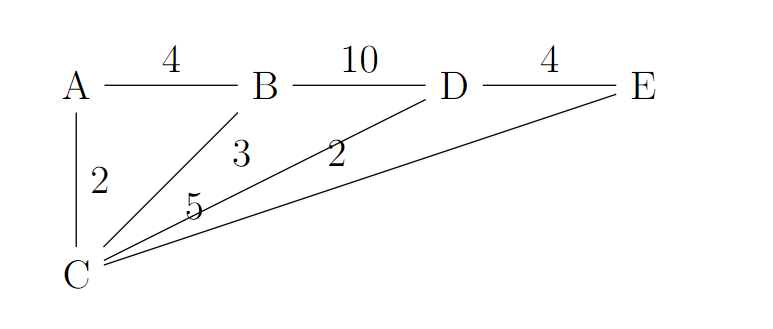
\includegraphics[width=0.5\textwidth]{images/weighted_graph_example.png}
    \caption{Example of a weighted graph}
    \label{fig:weighted_graph}
\end{figure}

If you start at vertex A, Dijkstra’s algorithm helps map out the shortest path to every other vertex, updating the route dynamically as it progresses from vertex to vertex.

\FloatBarrier
This approach not only makes Dijkstra's algorithm super efficient for these kinds of tasks but also a staple in computer science and operations research.


By applying Dijkstra's algorithm to the given graph, we can determine the shortest paths from vertex A to all other vertices and their respective distances.

\FloatBarrier
\textbf{Python Code Implementation of the algorithm above:}
\FloatBarrier
\begin{lstlisting}
import heapq

def dijkstra(graph, start):
    # Initialize distances
    distances = {vertex: float('inf') For vertex in graph}
    distances[start] = 0
    
    # Priority queue to store vertices with their tentative distances
    pq = [(0, start)]
    
    while pq:
        current_distance, current_vertex = heapq.heappop(pq)
        
        # Skip if the current distance is greater than the known distance
        if current_distance > distances[current_vertex]:
            continue
        
        # Explore neighboring vertices
        For neighbor, weight in graph[current_vertex].items():
            distance = current_distance + weight
            # Update distance if shorter path found
            if distance < distances[neighbor]:
                distances[neighbor] = distance
                heapq.heappush(pq, (distance, neighbor))
    
    Return distances

# Example graph representation
graph = {
    'A': {'B': 4, 'C': 2},
    'B': {'C': 5, 'D': 10},
    'C': {'D': 3, 'E': 2},
    'D': {'E': 4},
    'E': {}
}

# Start vertex
start_vertex = 'A'

# Run Dijkstra's algorithm
shortest_paths = dijkstra(graph, start_vertex)
print("Shortest paths from vertex", start_vertex)
For vertex, distance in shortest_paths.items():
    print("Vertex:", vertex, "- Distance:", distance)
    
\end{lstlisting}
\FloatBarrier

To provide an algorithmic example of the Minimum Spanning Tree (MST) method in graph theory, let's use Kruskal's algorithm. Kruskal's algorithm is a greedy algorithm that finds a minimum spanning tree For a connected, undirected graph. The basic idea is to sort the edges of the graph by weight and then add them to the MST in increasing order of weight, while ensuring that no cycles are Formed. Here's the algorithmic description:

\begin{algorithm}[H]
\caption{Kruskal's Algorithm For Minimum Spanning Tree}
\begin{algorithmic}[1]
\Procedure{KruskalMST}{$G(V, E)$}
\State $T \gets \emptyset$ \Comment{Initialize the MST}
\State $E' \gets \text{sort}(E)$ \Comment{Sort edges by weight}
\For{$(u, v) \in E'$}
\If{$T \cup {(u, v)}$ Forms no cycle}
\State $T \gets T \cup {(u, v)}$ \Comment{Add edge to MST}
\EndIf
\EndFor
\State \textbf{Return} $T$ \Comment{Return the MST}
\EndProcedure
\end{algorithmic}
\end{algorithm}
\FloatBarrier
\textbf{Python Code equivalent For the algorithm above:}
\FloatBarrier
\begin{lstlisting}
class DisjointSet:
    def __init__(self, vertices):
        self.parent = {v: v For v in vertices}
        self.rank = {v: 0 For v in vertices}

    def find(self, v):
        if self.parent[v] != v:
            self.parent[v] = self.find(self.parent[v])
        Return self.parent[v]

    def union(self, u, v):
        root_u = self.find(u)
        root_v = self.find(v)
        if root_u == root_v:
            Return False
        if self.rank[root_u] < self.rank[root_v]:
            self.parent[root_u] = root_v
        elif self.rank[root_u] > self.rank[root_v]:
            self.parent[root_v] = root_u
        else:
            self.parent[root_v] = root_u
            self.rank[root_u] += 1
        Return True

def kruskal_mst(graph):
    vertices = set()
    edges = []
    For u, neighbors in graph.items():
        vertices.add(u)
        For v, weight in neighbors:
            edges.append((weight, u, v))
            vertices.add(v)
    disjoint_set = DisjointSet(vertices)
    mst = []
    edges.sort()
    For weight, u, v in edges:
        if disjoint_set.union(u, v):
            mst.append((u, v))
    Return mst

# Example usage:
graph = {
    'A': [('B', 2), ('C', 3)],
    'B': [('C', 4), ('D', 5)],
    'C': [('D', 2), ('F', 1), ('E', 7)],
    'D': [('E', 6)],
    'E': [('F', 8)],
    'F': []
}

minimum_spanning_tree = kruskal_mst(graph)
print("Minimum Spanning Tree:", minimum_spanning_tree)
\end{lstlisting}
\FloatBarrier
In this algorithm, $G(V, E)$ represents the input graph with vertices $V$ and edges $E$. The algorithm initializes an empty set $T$ to represent the MST and sorts the edges of the graph by weight. Then, it iterates through the sorted edges and adds each edge to the MST if adding it does not Form a cycle. This is typically checked using a disjoint-set data structure (Union-Find). Finally, the algorithm Returns the resulting MST $T$.

Let's illustrate Kruskal's algorithm with a graph:
\FloatBarrier
\begin{figure}[h]
    \centering
    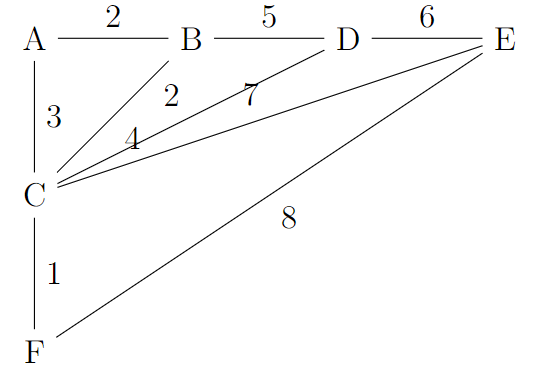
\includegraphics[width=0.5\textwidth]{images/Kruskal_algorithm_example.png}
    \caption{Weighted graph example}
    \label{fig:Kruskal_algorithm_graph}
\end{figure}
\FloatBarrier

Using Kruskal's algorithm, we start with the edge with weight $1 (C-F)$, then add edges with weights $2, 2, 3, 4, 5, and finally 6$ to Form the minimum spanning tree. The resulting MST is shown below:
\FloatBarrier
\begin{figure}[h]
    \centering
    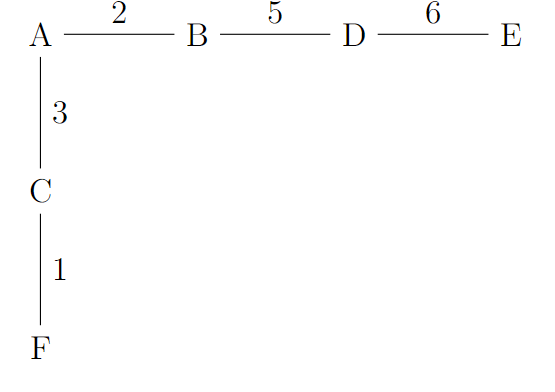
\includegraphics[width=0.5\textwidth]{images/Kruskal_algorithm_MST.png}
    \caption{Weighted graph example}
    \label{fig:Kruskal_algorithm_MST_graph}
\end{figure}
\FloatBarrier
This example demonstrates the application of Kruskal's algorithm to find a minimum spanning tree in a graph. The algorithm efficiently selects edges of minimum weight, ensuring that the resulting tree spans all vertices with the minimum total weight.

\subsubsection{Importance in Graph Theory}
Shortest paths and minimum spanning trees (MSTs) aren't just theoretical concepts; they're at the heart of solving practical problems in fields like transportation, communication, and logistics. They help us find efficient ways to navigate complex networks and optimize various systems.

\textbf{Shortest Paths}

Think of shortest paths as the most efficient route between any two points in a network. Whether it’s driving across the city or sending data across the internet, finding these paths efficiently is crucial for speeding things up and cutting down on costs.

\textbf{Everyday Applications of Shortest Paths}

\begin{itemize}
    \item \textbf{Navigation Systems}: They help your GPS find the quickest route, considering things like traffic and road closures.
    \item \textbf{Network Routing}: These algorithms keep your internet data zipping along the fastest routes, avoiding congestion.
    \item \textbf{Resource Allocation}: From deploying emergency services to managing delivery routes, shortest paths make sure resources are used effectively.
\end{itemize}

\textbf{Minimum Spanning Trees}

MSTs are all about connecting points in the most cost-effective way. Imagine setting up power lines or laying internet cables; MSTs guide where to run lines to connect all points with the least amount of cable.

\textbf{Practical Uses of Minimum Spanning Trees}

\begin{itemize}
    \item \textbf{Network Design}: Used to lay out communication networks or electrical grids efficiently, minimizing installation costs.
    \item \textbf{Circuit Layout}: Helps in designing circuits that use the least wire, making them cheaper to produce and simpler to maintain.
    \item \textbf{Clustering Analysis}: In data science, MSTs help identify natural groupings or patterns in data, useful for everything from market research to bioinformatics.
    \item \textbf{Spanning Tree Protocols}: These are crucial in networking, preventing loops and ensuring data flows smoothly across large networks.
\end{itemize}

Understanding shortest paths and MSTs isn't just academic—it's essential for optimizing and improving systems in nearly every area of our connected world.

\subsection{Borůvka's Algorithm}

Borůvka's algorithm is a classic approach to finding a minimum spanning tree (MST) in a graph. Created in 1926 by Otakar Borůvka, this algorithm is particularly good at building the most cost-effective network by gradually merging trees into a forest.

\subsubsection{Algorithm Overview}

Here’s how Borůvka's algorithm unfolds step-by-step:

\begin{enumerate}
    \item \textbf{Initialization}: Start with each vertex of the graph as its own separate tree.
    
    \item \textbf{Main Loop}:
        \begin{enumerate}
            \item \textbf{Find Cheapest Edge}: Identify the least expensive edge for each tree that connects it to another tree.
            \item \textbf{Merge Trees}: Add this cheapest edge to the MST and merge the trees connected by this edge into one.
        \end{enumerate}
        
    \item \textbf{Stopping Criterion}: Keep merging trees until there’s only one tree left, encompassing all vertices.
\end{enumerate}

The process effectively ensures that you gradually build up a single tree that spans all the points in your network, doing so in the most cost-effective manner.

\textbf{Mathematical Breakdown}:

Imagine your graph \( G = (V, E) \), with \( V \) being vertices and \( E \) the edges. Borůvka’s algorithm will build the MST \( T = (V, E_T) \), where \( E_T \) includes only those edges that form the minimum spanning tree.

Here's the drill:

\begin{itemize}
    \item \textbf{Initialization}: Every vertex \( v \) is a standalone tree, \( T_v = (\{v\}, \emptyset) \).
    
    \item \textbf{Main Loop}: During each iteration, the cheapest connecting edge \( (u, v) \) between any two trees \( T_u \) and \( T_v \) is added to \( E_T \), merging \( T_u \) and \( T_v \).
    
    \item \textbf{Stopping Criterion}: The process stops once all vertices are interconnected by one comprehensive tree, marking the completion of the MST \( T \).
\end{itemize}

Borůvka’s algorithm is not just theoretically interesting; it’s also practically efficient, typically running in \( O(E \log V) \) time. This makes it a robust choice for constructing minimum spanning trees in various applications, from network design to operational planning.

\FloatBarrier
\textbf{Python Code Implementation of Boruvka's Algorithm:}
\FloatBarrier
\begin{lstlisting}
class Subset:
    def __init__(self, parent, rank):
        self.parent = parent
        self.rank = rank

def find(subsets, i):
    if subsets[i].parent != i:
        subsets[i].parent = find(subsets, subsets[i].parent)
    Return subsets[i].parent

def union(subsets, x, y):
    xroot = find(subsets, x)
    yroot = find(subsets, y)

    if subsets[xroot].rank < subsets[yroot].rank:
        subsets[xroot].parent = yroot
    elif subsets[xroot].rank > subsets[yroot].rank:
        subsets[yroot].parent = xroot
    else:
        subsets[yroot].parent = xroot
        subsets[xroot].rank += 1

def boruvka_mst(graph):
    result = []
    subsets = []
    V = len(graph)
    
    For v in range(V):
        subsets.append(Subset(v, 0))

    while len(result) < V - 1:
        cheapest = [Subset(-1, float('inf'))] * V

        For u, v, weight in graph:
            set1 = find(subsets, u)
            set2 = find(subsets, v)

            if set1 != set2 and weight < cheapest[set1].rank:
                cheapest[set1] = Subset(set2, weight)

        For node in range(V):
            if cheapest[node].parent != -1:
                u = node
                v = cheapest[node].parent
                result.append((u, v, cheapest[node].rank))
                union(subsets, u, v)

    Return result

# Example usage:
graph = [(0, 1, 10), (0, 2, 6), (0, 3, 5), (1, 3, 15), (2, 3, 4)]
print("Minimum Spanning Tree edges:")
print(boruvka_mst(graph))
\end{lstlisting}
\subsubsection{Historical Significance}

Borůvka's algorithm is a pioneer in graph theory, introduced by Otakar Borůvka in 1926 to address the electrical grid network problem. This early algorithm marked a significant milestone, advancing the understanding of graph structures and paving the way for future research in algorithm design. 

Though today we might lean towards Prim's or Kruskal's algorithms for most applications, Borůvka's approach was groundbreaking at the time, offering a systematic method to tackle minimum spanning tree (MST) problems efficiently. It's a testament to the ingenuity of early 20th-century mathematicians and their contributions to the computational methods we rely on today.

\subsubsection{Comparison with Prim's and Kruskal's Algorithms}

When we look at Borůvka's algorithm alongside Prim's and Kruskal's, we gain insight into different strategies for constructing MSTs and their suitability for various graph scenarios:

\begin{enumerate}
    \item \textbf{Edge Selection Strategy:}
    \begin{itemize}
        \item \textbf{Borůvka's Algorithm:} Adds the lightest edge connecting separate components in each round.
        \item \textbf{Prim's Algorithm:} Focuses on expanding the MST from a chosen starting vertex by adding the lightest adjacent edge not already in the tree.
        \item \textbf{Kruskal's Algorithm:} Selects the overall lightest edge that doesn’t form a cycle, progressively building the MST.
    \end{itemize}

    \item \textbf{Time Complexity:}
    \begin{itemize}
        \item All three algorithms can operate within \(O(E \log V)\), but Borůvka's is particularly swift with sparse graphs due to its component-focused approach.
        \item Prim's and Kruskal's time efficiencies often depend on the underlying data structures used.
    \end{itemize}

    \item \textbf{Space Complexity:}
    \begin{itemize}
        \item Similar space requirements across the board: Borůvka's and Kruskal's might need slightly more space to manage components or sets, while Prim's generally sticks to \(O(V)\) with priority queues.
    \end{itemize}

    \item \textbf{Performance Considerations:}
    \begin{itemize}
        \item Borůvka's excels in sparse graphs with many vertices.
        \item Prim's is preferred for dense graphs where its edge selection is most efficient.
        \item Kruskal's is valued for its simplicity and robust performance across diverse graph types.
    \end{itemize}
\end{enumerate}

Choosing between Borůvka's, Prim's, and Kruskal's often boils down to the specific characteristics of the graph in question and the particular performance needs of the application.

\section{Huffman Coding}
\subsection{Problem Definition}
Huffman coding is a method used to encode characters based on their frequencies. The objective is to minimize the total encoding length while ensuring unique decodability. In this algorithm, characters with higher frequencies are assigned shorter codes compared to characters with lower frequencies. 


\subsection{Huffman Algorithm: A Greedy Approach}

The method is used For lossless data compression. It works by assigning variable-length codes to input characters, with shorter codes assigned to more frequent characters. The core idea behind Huffman coding is to construct an optimal prefix-free binary tree that represents the encoding.
\FloatBarrier
\textbf{Algorithm Overview:}
\FloatBarrier
\begin{algorithm}
\caption{Huffman Coding Algorithm}
\textbf{Algorithm Overview:}
\FloatBarrier
\begin{algorithmic}[1]
\Procedure{HuffmanCoding}{}
\State $Q \gets$ priority queue of characters based on frequencies
\While{$|Q| > 1$}
    \State $x \gets$ extractMin($Q$)
    \State $y \gets$ extractMin($Q$)
    \State $z \gets$ new internal node with frequency $x$ + $y$
    \State $z \text{.left} \gets x$
    \State $z \text{.right} \gets y$
    \State insert($Q, z$)
\EndWhile
\State \textbf{Return} root of the Huffman tree
\EndProcedure
\end{algorithmic}

\end{algorithm}
\FloatBarrier
\textbf{Python Implementation of the Huffman Algorithm:}
\FloatBarrier
\begin{lstlisting}
import heapq

class Node:
    def __init__(self, char, frequency):
        self.char = char
        self.frequency = frequency
        self.left = None
        self.right = None

def huffman_coding(char_freq):
    pq = [(freq, Node(char, freq)) For char, freq in char_freq.items()]
    heapq.heapify(pq)
    
    while len(pq) > 1:
        freq1, node1 = heapq.heappop(pq)
        freq2, node2 = heapq.heappop(pq)
        
        merged_node = Node(None, freq1 + freq2)
        merged_node.left = node1
        merged_node.right = node2
        
        heapq.heappush(pq, (freq1 + freq2, merged_node))
        
    Return pq[0][1]  # Root of Huffman tree

# Example usage
char_freq = {'a': 5, 'b': 9, 'c': 12, 'd': 13, 'e': 16, 'f': 45}
root = huffman_coding(char_freq)

\end{lstlisting}

\subsection{Optimality and Application in Data Compression}
The Huffman algorithm is considered optimal For constructing prefix-free binary trees in terms of minimizing the average encoding length of symbols. This optimality is achieved through a greedy approach, where decisions are made at each step based solely on the local optimal choice.

\subsection{Understanding the Huffman Algorithm}

\textbf{Algorithmic Overview}
\FloatBarrier
The Huffman algorithm is a slick method for creating prefix-free binary trees. It's designed to minimize the average encoding length of symbols, making it highly efficient for data compression. This efficiency comes from its greedy approach, which means at each step, it makes the choice that seems the best at that moment without considering the bigger picture.

\textbf{Proof of Optimality}

\textit{How do we know it's optimal?} The Huffman algorithm is proven to generate the most efficient prefix-free binary tree possible for a given set of symbols and their frequencies.

\textbf{The proof goes like this:}
\begin{enumerate}
    \item \textit{Unique Codes:} It starts by ensuring no code is a prefix of another, which is crucial for clear decoding.
    
    \item \textit{Assume a Better Tree Exists:} Imagine there's a better tree than what Huffman creates, called $T'$. This tree supposedly has a shorter average encoding length.
    
    \item \textit{Compare Frequencies:} Look at the least frequent symbols. Huffman’s process always combines the least frequent symbols first, so the frequencies at the leaves of $T$ must be at least as low as those in $T'$.
    
    \item \textit{Swap and Compare:} Swap in the leaves from Huffman’s tree into $T'$. If $T'$ still had a shorter length, it would now be the same as Huffman’s, contradicting our assumption that $T'$ was better.
\end{enumerate}

This contradiction shows that Huffman’s tree must indeed be optimal.

\textbf{Using Huffman for Data Compression}
\FloatBarrier
In practical terms, the Huffman algorithm shines in data compression scenarios:
\begin{itemize}
    \item \textit{Encoding:} Symbols that occur more frequently get shorter codes, which means less space.
    \item \textit{Decoding:} To get back the original data, just walk through the Huffman tree according to the encoded bits until hitting a leaf node.
\end{itemize}

\textbf{Greedy Mechanics}
The algorithm continuously merges the two least frequent nodes until only one remains. This not only simplifies the tree’s construction but ensures that frequently appearing symbols use shorter, quicker paths in the tree.

\textbf{Encoding and Decoding Steps}
\begin{itemize}
    \item \textit{Encoding Process:} Start at the root and traverse to the leaves. Append '0' for left turns and '1' for right turns, and voilà—you have your encoded data.
    \item \textit{Decoding Process:} Begin at the root and use the encoded bits to navigate to the leaves. Each leaf corresponds to a symbol, and traversing the tree decodes your data.
\end{itemize}

The Huffman algorithm not only exemplifies a beautiful use of greedy algorithms but also significantly impacts data storage and transmission efficiency.

\textbf{Example}

Let's consider an example of using the Huffman algorithm For data compression:

Suppose we have the following input data consisting of symbols and their frequencies:
\FloatBarrier
\[
\begin{array}{|c|c|}
\hline
\text{Symbol} & \text{Frequency} \\
\hline
A & 5 \\
B & 9 \\
C & 12 \\
D & 13 \\
E & 16 \\
F & 45 \\
\hline
\end{array}
\]
\FloatBarrier
After applying the Huffman algorithm, we obtain the following binary codes For each symbol:
\FloatBarrier
\[
\begin{array}{|c|c|}
\hline
\text{Symbol} & \text{Huffman Code} \\
\hline
A & 110 \\
B & 111 \\
C & 00 \\
D & 01 \\
E & 10 \\
F & 10 \\
\hline
\end{array}
\]
\FloatBarrier
Using these codes, we can compress the input data by replacing each symbol with its corresponding Huffman code. During decompression, the original data can be reconstructed by decoding the compressed binary data using the Huffman tree.

The Huffman algorithm's greedy approach ensures that the resulting encoding is close to optimal, making it a widely used method For data compression in various applications.

\section{Challenges and Future Directions}

Greedy algorithms are popular due to their simplicity and efficiency in solving optimization problems. However, they do have limitations and offer exciting avenues for future research.

\textbf{Optimality and the Greedy Choice Property}

A key challenge with greedy algorithms is ensuring they lead to the best possible solution globally, not just locally. To guarantee that a series of optimal choices leads to an overall optimal solution, detailed mathematical proofs and analysis are often necessary. This aspect requires deep understanding and innovative approaches to ensure that the greedy steps align perfectly with global objectives.

\textbf{Complexity Analysis}

While greedy algorithms are often efficient, understanding their computational limits is crucial. Some problems might push greedy algorithms into exponential time complexities, which calls for a clear analysis to identify such scenarios and possibly refine the algorithmic approach for practical applications.

\textbf{Handling Constraints and Variants}

Real-world problems often come with a twist—additional constraints or unique conditions that standard greedy algorithms might not initially accommodate. Researchers are actively working on ways to adapt greedy methods to manage these complexities effectively, such as integrating capacity limits or precedence rules without losing the inherent efficiency of the greedy approach.

\textbf{Robustness and Adaptability}

Another area of focus is making greedy algorithms more robust and adaptable to changes. Whether it’s a shift in input data or evolving problem conditions, enhancing greedy algorithms to be more dynamic and responsive is a critical research direction. Techniques like online and incremental learning are part of this effort, aiming to refine solutions continuously as new data emerges.

\textbf{Hybrid and Metaheuristic Approaches}

To overcome some inherent limitations of greedy algorithms, there’s growing interest in hybrid or metaheuristic methods. These approaches combine greedy strategies with other optimization frameworks, such as dynamic programming or evolutionary algorithms, to enhance performance and scalability. For example, integrating a greedy method with simulated annealing or genetic algorithms can provide more robust solutions across a broader range of problems.

\textbf{Applications in Machine Learning and Artificial Intelligence}

With the surge in machine learning and AI, greedy algorithms are increasingly employed to solve various optimization tasks, from feature selection in large datasets to decision-making in reinforcement learning. The future here involves developing specialized greedy approaches that are finely tuned to the nuances and demands of AI applications.

In conclusion, while greedy algorithms already offer powerful solutions across many domains, pushing their boundaries through innovative research and application-specific adaptations will further enhance their utility and effectiveness in tackling complex, real-world challenges.

\subsection{Beyond Greediness: Hybrid Algorithms}

Hybrid greedy algorithms blend the straightforwardness of greedy methods with other optimization techniques to enhance solution quality, scalability, and robustness. This fusion aims to sidestep the limitations of pure greedy approaches, achieving superior performance in tackling complex problems.

\textbf{Integration of Dynamic Programming}

A popular tactic in hybrid algorithms is weaving in dynamic programming. This technique optimizes problems with overlapping subproblems by memorizing intermediate results, which helps in circumstances where a greedy-only approach might falter. Although this might increase computational demands, the payoff in solution quality often justifies the extra effort.

\textbf{Local Search and Metaheuristic Techniques}

Hybrid algorithms often employ local search or metaheuristic strategies to refine greedy-generated solutions. Local search tweaks a current solution by exploring nearby possibilities, improving it incrementally. Metaheuristics like simulated annealing or genetic algorithms, on the other hand, offer broader exploration capabilities that can enhance the greedy groundwork by exploring more of the solution space.

\textbf{Genetic Algorithms and Evolutionary Strategies}

Genetic algorithms (GAs) and evolutionary strategies (ES) mimic natural selection processes to evolve solutions, making them great partners for greedy methods. These strategies can start from greedy-generated solutions and evolve them using operations like crossover and mutation, efficiently balancing between solution exploration and exploitation.

\textbf{Adaptive and Learning-based Approaches}

Incorporating adaptive strategies or machine learning into greedy algorithms can significantly boost their adaptability and effectiveness. Adaptive algorithms modify their tactics based on real-time feedback, optimizing their approach to changing conditions or problems. Machine learning, meanwhile, can help model and predict problem dynamics, informing better greedy choices and refining solutions over time.

\textbf{Applications and Future Directions}

Hybrid greedy algorithms are gaining ground in fields like combinatorial optimization, scheduling, and even machine learning. Looking ahead, we can expect further specialization of these hybrids for particular problems, innovative combinations of techniques, and enhanced learning-based strategies to improve scalability and solution accuracy. As technology advances, hybrid algorithms are set to become even more central in solving the intricate challenges of optimization and pushing the envelope in algorithmic research and practical applications.


\subsection{Theoretical Limits of Greedy Algorithms}

Greedy algorithms are popular for their simplicity and efficiency but sometimes fall short of delivering optimal solutions. Recognizing the boundaries of what greedy algorithms can achieve is essential for both applying them effectively and understanding where they might falter.

\textbf{Optimality and Greedy Choice Property}

The core of greedy algorithms—the greedy choice property—suggests that the best choice at each step will lead to the best overall solution. However, this isn't always the case. Greedy algorithms may lack the foresight needed to navigate towards the global optimum, often settling for locally optimal solutions instead.

\textbf{Counterexamples and Proof of Suboptimality}

Exploring counterexamples where greedy algorithms fail provides valuable insights into their limitations. These examples help pinpoint specific scenarios where the algorithm's local decisions do not align with the optimal global strategy, serving as proof of their potential suboptimality.

\textbf{Proof Techniques and Complexity Analysis}

Through mathematical proofs and complexity analysis, we can rigorously assess where and why greedy algorithms might underperform. This analysis not only confirms the situations in which these algorithms are effective but also highlights where they struggle, particularly in complex scenarios that demand a more nuanced approach.

\textbf{Examples of NP-Hard Problems}

Greedy algorithms often struggle with NP-hard problems, such as the traveling salesman problem or the knapsack problem. These problems are notoriously difficult to solve within polynomial time, and greedy methods may fail to find the best solutions efficiently, if at all.

\textbf{Trade-offs and Approximation Algorithms}

Despite these challenges, greedy algorithms are invaluable in scenarios where perfect solutions are less crucial than finding good enough solutions quickly. They often form the backbone of approximation algorithms that offer a pragmatic balance between optimality and computational efficiency.

\textbf{Challenges and Open Questions}

The limitations of greedy algorithms pose significant challenges and raise important questions in optimization theory. Ongoing research is crucial to develop more sophisticated algorithms that can handle the complexity of real-world problems more effectively, possibly by combining greedy principles with other algorithmic strategies.

\subsection{Emerging Research Areas and Open Problems}

The study of greedy algorithms continues to evolve, with several research areas offering opportunities for further exploration:

\textbf{Online and Streaming Algorithms}

In the realm of online and streaming algorithms, greedy methods face the challenge of making optimal decisions with incomplete information. Research is ongoing into how these algorithms can adapt dynamically to new data and changing conditions.

\textbf{Adversarial and Robust Optimization}

The robustness of greedy algorithms against adversarial inputs is another area of active investigation. Enhancing these algorithms to withstand strategic disruptions could greatly improve their reliability and applicability.

\textbf{Greedy Techniques in Machine Learning and AI}

As AI and machine learning continue to advance, greedy algorithms are being tailored to tackle large-scale data and complex decision-making processes. This involves integrating greedy strategies with more sophisticated machine learning models to optimize performance.

\textbf{Greedy Algorithms for Quantum Computing}

Quantum computing presents a novel frontier for greedy algorithms. Research in this area focuses on leveraging quantum mechanics to enhance the performance of greedy methods beyond the capabilities of classical computing.

\textbf{Multi-objective and Pareto-Optimal Greedy Algorithms}

Addressing multi-objective optimization problems with greedy algorithms involves finding a balance between competing goals. This research seeks to refine greedy approaches to better manage these complexities and achieve Pareto-optimal solutions.

\textbf{Algorithmic Fairness and Social Good}

Finally, the societal impacts of greedy algorithms, particularly their role in resource allocation and decision-making, underscore the need for fairness-aware optimization strategies. This research aims to mitigate biases and ensure that algorithmic decisions promote equity and social good.

In summary, while greedy algorithms have proven effective in many contexts, the breadth of ongoing research highlights both their potential and the challenges they face. As computational techniques advance, so too will the sophistication and applicability of greedy algorithms.

\section{Conclusion}

\subsection{Summary of Key Points}
Greedy algorithms are essential in solving various optimization challenges across multiple domains. Here, we recap their characteristics, benefits, limitations, and the breadth of their applications.

\textbf{Characteristics of Greedy Algorithms}

Known for their straightforward approach, greedy algorithms make local optimal choices at each step, aiming for a near-optimal solution with minimal computational efforts. Their effectiveness largely depends on the specific problem's structure and the greedy criteria applied.

\textbf{Advantages of Greedy Algorithms}

The primary advantage of greedy algorithms lies in their efficiency, often demonstrating linear or logarithmic complexity. This makes them particularly useful for large-scale problems. Additionally, their ease of implementation and ability to handle dynamic data makes them attractive for real-time applications.

\textbf{Limitations of Greedy Algorithms}

Despite their strengths, greedy algorithms can sometimes miss the global optimum due to their lack of foresight, making them unsuitable for problems with complex dependencies or conflicting objectives. Their effectiveness varies greatly depending on the problem at hand.

\textbf{Theoretical and Practical Implications}

Theoretical studies provide a deep understanding of when and how greedy algorithms work best, using formal proofs and mathematical models. Practically, they are applied in fields like computer science, engineering, and bio informatics for tasks such as scheduling, routing, and data compression.

\textbf{Future Directions in Greedy Algorithm Research}

Looking ahead, research will likely aim to overcome the inherent limitations of greedy algorithms by developing hybrid strategies, incorporating adaptive elements, and applying advanced computational methods. Additionally, there's a growing push to integrate ethical considerations into algorithm design to ensure fairness and transparency.

\subsection{The Role of Greedy Algorithms in Computer Science}

Greedy algorithms are pivotal in computer science, offering effective solutions to a wide array of optimization problems. Their role extends from theoretical formulations to practical applications, impacting various areas of technology and computation.

\textbf{Significance and Applications}

In computer science, greedy algorithms simplify complex problem-solving by providing efficient solutions for graph-based computations, data compression, and resource management. They are fundamental in designing algorithms for networking, system optimization, and beyond.

\textbf{Innovative Research Directions}

Future research will continue to explore new ways to enhance the performance and applicability of greedy algorithms. This includes hybrid approaches, leveraging machine learning techniques, and ensuring algorithms are robust and adaptable to evolving computational environments. The focus will also be on addressing ethical concerns to mitigate biases and improve the societal impact of these algorithms.

In conclusion, greedy algorithms remain invaluable tools in computational sciences. With ongoing advancements in technology and methodology, they hold the potential to solve increasingly complex problems, continually expanding their utility and effectiveness in various applications.


\section{Exercises and Problems}
In this section, we will delve into a variety of exercises and problems that are designed to test and strengthen your understanding of greedy algorithm techniques. Greedy algorithms are a powerful tool in the field of computer science and are used to solve optimization problems by making a sequence of choices, each of which looks the best at the moment.

The exercises and problems are divided into two main categories: conceptual questions and practical coding problems. The conceptual questions are meant to test your theoretical understanding of greedy algorithms, while the practical coding problems are intended to give you hands-on experience in implementing these algorithms in Python.

\subsection{Conceptual Questions to Test Understanding}
Conceptual questions are crucial for ensuring that you have a solid grasp of the fundamental principles and ideas underlying greedy algorithms. These questions are designed to make you think deeply about the properties and behaviors of greedy algorithms and how they can be applied to various problems.

\begin{itemize}
    \item What is a greedy algorithm, and how does it differ from other algorithmic paradigms such as dynamic programming and divide-and-conquer?
    \item Explain the concept of "optimal substructure" and how it applies to greedy algorithms.
    \item Describe the "greedy choice property" and provide an example of a problem where this property is essential.
    \item Discuss a situation where a greedy algorithm might fail to produce an optimal solution. Provide an example to illustrate your point.
    \item How can you prove that a greedy algorithm provides an optimal solution for a given problem? Outline the steps involved in such a proof.
    \item Compare and contrast the use of greedy algorithms in solving the Minimum Spanning Tree (MST) problem using Kruskal's and Prim's algorithms.
    \item Explain the role of greedy algorithms in Huffman coding. How does the greedy approach ensure that the resulting code is optimal?
    \item Discuss the time and space complexity considerations when implementing a greedy algorithm. How do these compare to other algorithmic approaches?
    \item Provide a real-world example where a greedy algorithm is used and explain why it is suitable for that particular problem.
\end{itemize}

\subsection{Practical Coding Problems to Strengthen Skills}
Practical coding problems help reinforce the concepts learned by applying them to real-world scenarios. In this subsection, we present several coding problems related to greedy algorithms. Each problem is accompanied by a detailed solution and Python code implementation.

\begin{itemize}
    \item \textbf{Problem 1: Coin Change Problem}
    \begin{itemize}
        \item \textbf{Description:} Given an infinite supply of coins of different denominations, find the minimum number of coins needed to make a given amount of money.
        \item \textbf{Algorithm:} Use a greedy algorithm to select the largest denomination coin that does not exceed the remaining amount.
    \end{itemize}
    
    \begin{algorithm}
    \caption{Greedy Coin Change Algorithm}
    \begin{algorithmic}[1]
    \Require A list of coin denominations $C = \{c_1, c_2, ..., c_k\}$ sorted in descending order, and an amount $A$.
    \Ensure The minimum number of coins needed to make the amount $A$.
    \State $num\_coins \leftarrow 0$
    \For{each coin $c$ in $C$}
        \While{$A \geq c$}
            \State $A \leftarrow A - c$
            \State $num\_coins \leftarrow num\_coins + 1$
        \EndWhile
    \EndFor
    \Return $num\_coins$
    \end{algorithmic}
    \end{algorithm}

    \FloatBarrier
    \begin{lstlisting}
def coin_change(coins, amount):
    num_coins = 0
    for coin in coins:
        while amount >= coin:
            amount -= coin
            num_coins += 1
    Return num_coins

coins = [25, 10, 5, 1]
amount = 63
print(f"Minimum number of coins: {coin_change(coins, amount)}")
    \end{lstlisting}
    \FloatBarrier

    \item \textbf{Problem 2: Activity Selection Problem}
    \begin{itemize}
        \item \textbf{Description:} Given a set of activities with start and finish times, select the maximum number of activities that can be performed by a single person, assuming that a person can only work on a single activity at a time.
        \item \textbf{Algorithm:} Sort activities by their finish times. Select the activity that finishes first, then select the next activity that starts after the current one finishes.
    \end{itemize}

    \begin{algorithm}
    \caption{Greedy Activity Selection Algorithm}
    \begin{algorithmic}[1]
    \Require A list of activities with their start and finish times $(s_1, f_1), (s_2, f_2), ..., (s_n, f_n)$ sorted by finish times.
    \Ensure The maximum number of non-overlapping activities.
    \State Let $A \leftarrow \emptyset$
    \State $A \leftarrow A \cup \{1\}$ \Comment{Select the first activity}
    \State $j \leftarrow 1$
    \For{$i \leftarrow 2$ to $n$}
        \If{$s_i \geq f_j$}
            \State $A \leftarrow A \cup \{i\}$
            \State $j \leftarrow i$
        \EndIf
    \EndFor
    \Return $A$
    \end{algorithmic}
    \end{algorithm}

    \FloatBarrier
    \begin{lstlisting}
def activity_selection(activities):
    activities.sort(key=lambda x: x[1])  # Sort by finish times
    selected_activities = [activities[0]]
    last_finish_time = activities[0][1]
    
    for start, finish in activities[1:]:
        if start >= last_finish_time:
            selected_activities.append((start, finish))
            last_finish_time = finish
            
    Return selected_activities

activities = [(1, 3), (2, 4), (3, 5), (0, 6), (5, 7), (8, 9), (5, 9)]
selected = activity_selection(activities)
print(f"Selected activities: {selected}")
    \end{lstlisting}
    \FloatBarrier

    \item \textbf{Problem 3: Fractional Knapsack Problem}
    \begin{itemize}
        \item \textbf{Description:} Given the weights and values of $n$ items, put these items in a knapsack of capacity $W$ to get the maximum total value in the knapsack. You can break items to maximize the total value.
        \item \textbf{Algorithm:} Calculate the value-to-weight ratio for each item. Sort items by this ratio. Take as much as possible of the item with the highest ratio until the knapsack is full.
    \end{itemize}

    \begin{algorithm}
    \caption{Greedy Fractional Knapsack Algorithm}
    \begin{algorithmic}[1]
    \Require A list of items with their weights and values $(w_1, v_1), (w_2, v_2), ..., (w_n, v_n)$, and a knapsack capacity $W$.
    \Ensure The maximum total value in the knapsack.
    \State Calculate the value-to-weight ratio for each item.
    \State Sort items by their value-to-weight ratio in descending order.
    \State $total\_value \leftarrow 0$
    \For{each item $i$ in sorted order}
        \If{$W = 0$}
            \Return $total\_value$
        \EndIf
        \State $a \leftarrow \min(w_i, W)$
        \State $total\_value \leftarrow total\_value + a \times \frac{v_i}{w_i}$
        \State $W \leftarrow W - a$
    \EndFor
    \Return $total\_value$
    \end{algorithmic}
    \end{algorithm}

    \FloatBarrier
    \begin{lstlisting}
def fractional_knapsack(weights, values, capacity):
    index = list(range(len(values)))
    ratio = [v/w for v, w in zip(values, weights)]
    index.sort(key=lambda i: ratio[i], reverse=True)
    
    total_value = 0
    for i in index:
        if capacity == 0:
            break
        a = min(weights[i], capacity)
        total_value += a * ratio[i]
        capacity -= a
        
    Return total_value

weights = [10, 20, 30]
values = [60, 100, 120]
capacity = 50
print(f"Maximum value in knapsack: {fractional_knapsack(weights, values, capacity)}")
    \end{lstlisting}
    \FloatBarrier
\end{itemize}

\section{Further Reading and Resources}
To deepen your understanding of greedy algorithms, several resources are available that provide comprehensive insights and practical examples. These resources include books, survey papers, online courses, video lectures, research articles, and case studies. In the following subsections, we will explore these resources in greater detail to guide your further study.

\subsection{Books and Survey Papers}
Books and survey papers are invaluable For building a strong theoretical foundation in greedy algorithms. They often cover the essential concepts, mathematical proofs, and various applications of greedy algorithms.

\subsubsection*{Important Books}
\begin{itemize}
    \item \textbf{Introduction to Algorithms} by Thomas H. Cormen, Charles E. Leiserson, Ronald L. Rivest, and ClifFord Stein - This book, often referred to as CLRS, is a comprehensive textbook covering a wide range of algorithms, including greedy algorithms. It provides detailed explanations, mathematical proofs, and exercises.
    \item \textbf{Algorithm Design} by Jon Kleinberg and Éva Tardos - This book offers a clear and well-structured presentation of various algorithmic techniques, including a dedicated chapter on greedy algorithms with practical examples and exercises.
    \item \textbf{The Design and Analysis of Algorithms} by Dexter C. Kozen - This book provides a focused introduction to the design and analysis of algorithms, with a section dedicated to greedy algorithms, including proofs of correctness and complexity analysis.
\end{itemize}

\subsubsection*{Notable Survey Papers}
\begin{itemize}
    \item \textbf{A Survey of Greedy Algorithms} by David Pisinger - This paper provides an extensive survey of greedy algorithms, discussing their applications, performance, and theoretical underpinnings.
    \item \textbf{Greedy Algorithms For Optimization Problems} by Vazirani and Klein - This survey paper explores various optimization problems that can be efficiently solved using greedy algorithms, providing a thorough analysis of their performance and limitations.
\end{itemize}

\subsection{Online Courses and Video Lectures}
Online courses and video lectures are excellent resources For learning about greedy algorithms in a more interactive and engaging manner. They often include practical coding examples, quizzes, and assignments to reinforce learning.

\subsubsection*{Important Online Tutorials and Courses}
\begin{itemize}
    \item \textbf{Coursera: Algorithms Specialization by StanFord University} - This series of courses, taught by Tim Roughgarden, covers a wide range of algorithms, including a module on greedy algorithms with detailed explanations and programming assignments.
    \item \textbf{edX: Algorithmic Design and Techniques by UC San Diego} - This course offers a comprehensive introduction to various algorithmic techniques, including greedy algorithms, with practical examples and exercises.
    \item \textbf{Udacity: Intro to Algorithms} - This course provides an introduction to algorithmic techniques, including a section on greedy algorithms with interactive quizzes and coding challenges.
    \item \textbf{Khan Academy: Algorithms} - This series of video lectures includes a section on greedy algorithms, explaining the concepts with visual aids and step-by-step problem-solving examples.
\end{itemize}

\subsection{Research Articles and Case Studies}
Research articles and case studies provide detailed insights into specific applications and implementations of greedy algorithms. They often include experimental results and comparisons with other algorithmic techniques.

\subsubsection*{Research Articles}
\begin{itemize}
    \item \textbf{Greedy Algorithms For the Minimum Spanning Tree Problem} by Kruskal and Prim - These foundational papers introduce Kruskal's and Prim's algorithms For finding the minimum spanning tree, which are classic examples of greedy algorithms.
    \item \textbf{Approximation Algorithms For NP-hard Problems} by Vazirani - This paper discusses how greedy algorithms can be used to develop approximation algorithms For NP-hard problems, providing theoretical guarantees on their performance.
    \item \textbf{A Greedy Algorithm For the Set Cover Problem} by Chvatal - This paper presents a greedy algorithm For the set cover problem, including a detailed analysis of its approximation ratio.
\end{itemize}

\subsubsection*{Case Studies}
\begin{itemize}
    \item \textbf{Network Design and Optimization} - Case studies in this area often use greedy algorithms to optimize network design and routing, demonstrating their effectiveness in real-world scenarios.
    \item \textbf{Job Scheduling Problems} - Research articles and case studies on job scheduling problems frequently employ greedy algorithms to achieve efficient resource allocation and time management.
    \item \textbf{Data Compression Techniques} - Many data compression algorithms, such as Huffman coding, are based on greedy strategies. Case studies in this field illustrate how greedy algorithms can be applied to reduce data size effectively.
\end{itemize}

\FloatBarrier
\begin{lstlisting}[language=Python, caption=Python Implementation of Kruskal's Algorithm]
# Example: Kruskal's Algorithm For Minimum Spanning Tree

class DisjointSet:
    def __init__(self, vertices):
        self.parent = {v: v For v in vertices}
        self.rank = {v: 0 For v in vertices}

    def find(self, item):
        if self.parent[item] == item:
            Return item
        else:
            self.parent[item] = self.find(self.parent[item])
            Return self.parent[item]

    def union(self, set1, set2):
        root1 = self.find(set1)
        root2 = self.find(set2)
        
        if root1 != root2:
            if self.rank[root1] > self.rank[root2]:
                self.parent[root2] = root1
            else:
                self.parent[root1] = root2
                if self.rank[root1] == self.rank[root2]:
                    self.rank[root2] += 1

def kruskal(graph):
    edges = []
    For u in graph:
        For v, weight in graph[u]:
            edges.append((weight, u, v))
    edges.sort()
    
    ds = DisjointSet(graph.keys())
    mst = []
    
    For weight, u, v in edges:
        if ds.find(u) != ds.find(v):
            ds.union(u, v)
            mst.append((u, v, weight))
    Return mst

# Example graph represented as an adjacency list
graph = {
    'A': [('B', 1), ('C', 3)],
    'B': [('A', 1), ('C', 1), ('D', 6)],
    'C': [('A', 3), ('B', 1), ('D', 5)],
    'D': [('B', 6), ('C', 5)]
}

mst = kruskal(graph)
print("Edges in the Minimum Spanning Tree:")
For edge in mst:
    print(edge)
\end{lstlisting}
\FloatBarrier

\begin{algorithm}
\caption{Kruskal's Algorithm For Minimum Spanning Tree}
\begin{algorithmic}
\State \textbf{Input:} A graph $G = (V, E)$ with weights on edges
\State \textbf{Output:} A minimum spanning tree $T$
\State Sort all edges in non-decreasing order of their weight
\State Initialize $T$ as an empty set
\For{each edge $(u, v)$ in the sorted list}
    \If{$u$ and $v$ are in different sets}
        \State Add $(u, v)$ to $T$
        \State Union the sets containing $u$ and $v$
    \EndIf
\EndFor
\State \textbf{Return} $T$
\end{algorithmic}
\end{algorithm}
\end{document}